\section{Princípios de Avaliação da Segurança Web}

\subsection{Tipos de Testes de Penetração}

A avaliação da segurança em aplicações web recorre, frequentemente, a testes de penetração (\textit{pentesting}). Estes testes consistem na simulação controlada de ataques informáticos, com o objetivo de identificar vulnerabilidades que possam ser exploradas por atacantes. É uma prática fundamental em cibersegurança, pois permite analisar a capacidade de resistência de uma aplicação perante ameaças reais, sem comprometer o seu funcionamento.

Consoante o grau de acesso à aplicação, os testes de penetração podem ser classificados em três modelos principais:

\begin{flushleft}
\textbullet\ \textbf{Testes de Caixa-Preta (\textit{Black-box}):} Aqui o avaliador não tem qualquer informação interna sobre a aplicação, aproximando-se da perspetiva de um atacante externo. A análise é feita exclusivamente através da interação com a aplicação em execução, sem qualquer acesso ao código-fonte ou à documentação da arquitetura.

\vspace{0.4cm}

\textbullet\ \textbf{Testes de Caixa-Branca (\textit{White-box}):} Neste caso, o avaliador tem acesso total a todos os elementos do sistema, incluindo o código-fonte, bases de dados e configurações dos servidores. Permite uma análise exaustiva e é especialmente útil na deteção de falhas lógicas ou estruturais.

\vspace{0.4cm}

\textbullet\ \textbf{Testes de Caixa-Cinzenta (\textit{Grey-box}):} Este modelo híbrido trata-se de uma abordagem intermédia, em que o avaliador tem acesso parcial ao sistema. Por exemplo, poderá ter acesso ao código do \textit{frontend} ou a credenciais de utilizadores com permissões limitadas. A abordagem caixa-cinzenta representa um equilíbrio entre o realismo da caixa-preta e a profundidade da caixa-branca, sendo frequentemente considerada a mais eficiente em termos de custo-benefício em diversos cenários de teste.
\end{flushleft}

Estas abordagens são amplamente reconhecidas nas boas práticas de engenharia de software e de testes de segurança \cite{ref37}.

\subsection{Justificação da Abordagem Adotada: Caixa-Cinzenta (\textit{Grey-box})}

No âmbito deste projeto, a abordagem de caixa-cinzenta foi considerada a mais adequada, tendo em conta as restrições impostas pela plataforma Base44. Sendo uma solução \textit{no-code}, baseada em inteligência artificial, o acesso ao \textit{backend} e à configuração do servidor está bloqueado. No entanto, todo o código do lado do cliente (\textit{HTML}, \textit{CSS} e \textit{JavaScript}) está disponível, o que permite realizar uma análise focada no \textit{frontend}.

A imagem seguinte ajuda a visualizar, de forma esquemática, a abordagem adotada neste projeto.

\begin{figure}
    \centering
    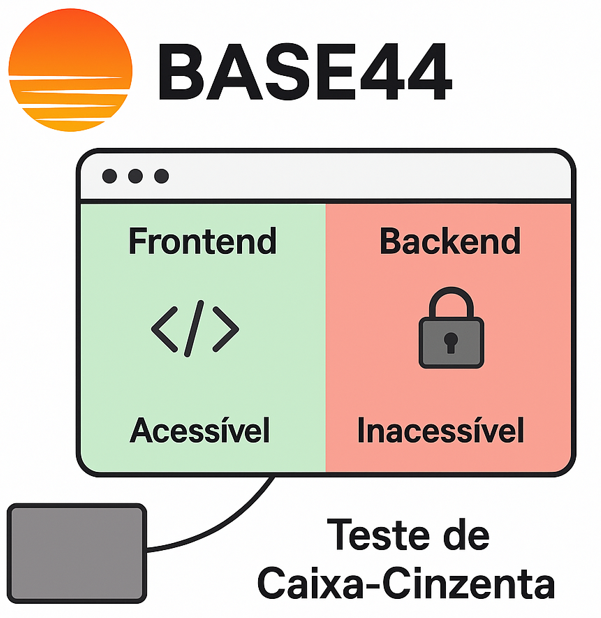
\includegraphics[width=0.4\linewidth]{imagens/diagrama.png}
    \caption{Representação esquemática da abordagem de caixa-cinzenta aplicada à Base44.}
    \label{fig:modelo_base44}
\end{figure}

Tal como representado na Figura~\ref{fig:modelo_base44}, apenas o \textit{frontend} da aplicação se encontra acessível para análise, enquanto o \textit{backend} permanece inacessível. Esta separação entre as duas camadas reflete as limitações impostas pela Base44 e ilustra bem a natureza da abordagem de caixa-cinzenta.

O diagrama reforça que, apesar do acesso restrito à infraestrutura do servidor, é possível aplicar técnicas de análise sobre os recursos disponíveis no lado do cliente. Esta abordagem equilibrada permite avaliar potenciais riscos de segurança de forma ética, segura e adequada ao contexto de plataformas \textit{no-code}.

A secção seguinte irá detalhar as ferramentas selecionadas, bem como a justificação técnica da sua utilização no âmbito do projeto.
